% ---------------------------------------------------------------------
\Needspace{8\baselineskip}\subsection{Programme du Raspberry Pi}

Le Raspberry est le cœur du système : c'est lui qui transforme des tensions en décisions. En écrivant ce programme, je veux pouvoir le tester avant même de recevoir le matériel. Je sépare donc ce qui dépend du matériel de ce qui n'en dépend pas, et je rends réglables depuis le dashboard toutes les valeurs qui risquaient de changer (seuils, durées, étalonnages).

Le programme est écrit en Python et se lance par \texttt{python server.py}. Il est découpé en trois fichiers, chacun avec un rôle clair : \texttt{arduino.py} parle à l'Arduino, \texttt{pilote.py} prend les décisions et \texttt{server.py} relie le tout, enregistre les mesures et sert le dashboard. Le fichier de décisions n'utilise aucun matériel : il peut être testé entièrement sur un ordinateur.

Cette sous-partie suit le trajet d'une mesure dans le programme : la boucle qui mesure et décide toutes les 10 secondes, puis le passage des tensions aux mesures, avec les calculs du pH, de l'EC et du niveau. Elle présente ensuite les décisions : la commande de la pompe principale selon la batterie et le soleil, et le dosage des engrais et du pH$-$ selon le légume. Elle se termine par les alertes et le journal.

\subsubsection*{La boucle de mesure}

Je choisis une période de \qty{10}{s} : c'est assez rapide pour réagir à un réservoir qui se vide, et assez lent pour laisser le temps de lire tous les capteurs (la sonde de température demande à elle seule près d'une seconde). L'ordre des étapes suit le raisonnement d'un jardinier : regarder, comprendre, décider, agir, puis noter ce qui a été fait.

Toutes les 10 secondes, le Raspberry enchaîne les mêmes étapes. Il commence par lire tous les capteurs (avec l'alternance pH / EC de la partie 8.2), puis il convertit les tensions en valeurs physiques (pH, \unit{\micro S/cm}, \%) avec l'étalonnage. Ensuite il calcule les cibles de pH et d'EC du légume, selon son stade, puis il décide de la pompe principale et des doses (parties 8.4, pompe principale et dosage). Enfin il renvoie l'état des pompes à l'Arduino, enregistre la mesure dans la base et met à jour l'écran.

Une erreur sur un capteur (fil débranché, module absent) n'arrête pas la boucle : la valeur manque simplement, et le module absent n'est réinterrogé qu'une minute plus tard pour ne pas ralentir les autres mesures.

\subsubsection*{Des tensions aux mesures}

Les capteurs ne donnent pas directement un pH ou une conductivité, mais une tension. Je reprends les formules des fabricants, et je place tous les réglages d'étalonnage dans le dashboard plutôt que dans le code : une sonde pH dérive avec le temps, et il faut pouvoir la réétalonner sans ouvrir le programme. Les capteurs analogiques donnent une tension ; le programme la transforme en grandeur utile. Les exemples ci-dessous reprennent les valeurs affichées dans les captures de la partie 8.5.

\naturecalc{théorie (formule démontrée, valeurs de fiches techniques et hypothèses ; rien de mesuré)}
\begin{demonstration}[pH à partir de la tension]
\resultat{\mathrm{pH} \approx 5{,}97}
La sonde est étalonnée dans deux solutions tampon : $U_7 = \qty{1500}{mV}$ à pH 7 et $U_4 = \qty{2032}{mV}$ à pH 4. J'admets que le pH est une fonction affine de la tension $U$ lue, en millivolts :
\[
\mathrm{pH} = a\,U + b
\]
Les deux solutions tampon donnent deux équations :
\begin{align*}
7 &= a\,U_7 + b\\
4 &= a\,U_4 + b
\end{align*}
En soustrayant la seconde à la première, $b$ disparaît :
\begin{align*}
7 - 4 &= a\,(U_7 - U_4)\\
a &= \frac{4-7}{U_4 - U_7}
\end{align*}
Je remplace $b$ en utilisant la première équation, $b = 7 - a\,U_7$ :
\begin{align*}
\mathrm{pH} &= a\,U + 7 - a\,U_7\\
\mathrm{pH} &= 7 + (U - U_7)\times\frac{4-7}{U_4 - U_7}
\end{align*}
Pour $U = \qty{1683}{mV}$ :
\begin{align*}
U_4 - U_7 &= \qty{2032}{mV} - \qty{1500}{mV} = \qty{532}{mV}\\
\mathrm{pH} &= 7 + (\qty{1683}{mV} - \qty{1500}{mV})\times\frac{-3}{\qty{532}{mV}}\\
\mathrm{pH} &= 7 - \frac{\qty{183}{mV}\times 3}{\qty{532}{mV}}\\
\mathrm{pH} &= 7 - 1{,}03\\
\mathrm{pH} &\approx 5{,}97
\end{align*}
Le résultat est arrondi au centième.
\end{demonstration}

\naturecalc{théorie (formule démontrée, valeurs de fiches techniques et hypothèses ; rien de mesuré)}
\begin{demonstration}[conductivité ramenée à \qty{25}{\celsius}]
\resultat{\mathrm{EC}_{25} \approx \qty{1467}{\micro S/cm}}
La conductivité d'une eau est la conductance mesurée entre deux électrodes, multipliée par la constante de cellule $K$ de la sonde (en cm$^{-1}$, rapport de la distance entre électrodes à leur surface). Cet exemple reprend la sonde du système de départ, la DFR0300 (la formule de la sonde fabriquée est en partie 7.7). La carte de la sonde DFR0300 transforme cette conductance en une tension $U$ proportionnelle. La conductivité brute est donc proportionnelle à $U$ et à $K$. Pour cette carte, le constructeur donne le coefficient de proportionnalité $\dfrac{1000}{820 \times 200}$, avec $U$ en millivolts et $K = 1$ :
\[
\mathrm{EC} = \frac{1000 \times U}{820 \times 200}\times K
\]
La conductivité augmente avec la température $T$ de l'eau (en \unit{\celsius}). J'admets une variation affine de $\alpha = \qty{1,85}{\percent}$ par degré (valeur du programme du dashboard ; la partie 7 prend \qty{2}{\percent}, valeur usuelle : l'écart de \qty{0,15}{\percent} par degré change l'EC de moins de \qty{1}{\percent} pour \qty{3}{\celsius} d'écart avec \qty{25}{\celsius}, sans effet sur le dosage) autour de \qty{25}{\celsius} :
\[
\mathrm{EC} = \mathrm{EC}_{25}\,\bigl[1 + \alpha\,(T - 25)\bigr]
\]
En isolant $\mathrm{EC}_{25}$, la conductivité ramenée à \qty{25}{\celsius}, on obtient :
\[
\mathrm{EC}_{25} = \frac{\mathrm{EC}}{1 + 0{,}0185\,(T - 25)}
\]
Pour $U = \qty{229}{mV}$ et $T = \qty{22,4}{\celsius}$ :
\begin{align*}
\mathrm{EC} &= \frac{1000 \times 229}{820 \times 200}\ \unit{mS/cm} = \frac{229000}{164000}\ \unit{mS/cm}\\
\mathrm{EC} &\approx \qty{1,396}{mS/cm}\\
1 + 0{,}0185 \times (22{,}4 - 25) &= 1 - 0{,}0481 = 0{,}9519\\
\mathrm{EC}_{25} &= \frac{\qty{1,396}{mS/cm}}{0{,}9519}\\
\mathrm{EC}_{25} &\approx \qty{1,467}{mS/cm} = \qty{1467}{\micro S/cm}
\end{align*}
\end{demonstration}

\naturecalc{théorie (formule démontrée, valeurs de fiches techniques et hypothèses ; rien de mesuré)}
\begin{demonstration}[niveau du réservoir]
\resultat{\text{niveau} = \qty{77,5}{\percent}\ \text{pour}\ R = \qty{760}{\ohm}}
Le ruban eTape\ix{23} est une résistance $R$ (en ohms) qui diminue quand l'eau monte. Il est placé en série avec une résistance de \qty{560}{\ohm}, sous \qty{5}{V} (\qty{5000}{mV}) : la tension $U$ lue entre les deux (en millivolts) est celle aux bornes du ruban. C'est un pont diviseur :
\[
U = 5000 \times \frac{R}{R + 560}
\]
Je multiplie par $R + 560$, puis je regroupe les termes en $R$ :
\begin{align*}
U\,(R + 560) &= 5000\,R\\
560\,U &= 5000\,R - U\,R\\
560\,U &= R\,(5000 - U)\\
R &= 560 \times \frac{U}{5000 - U}
\end{align*}
Le niveau $N$ est ensuite placé entre les deux étalonnages, $R_{\mathrm{vide}} = \qty{2000}{\ohm}$ (réservoir vide, $0\,\%$) et $R_{\mathrm{plein}} = \qty{400}{\ohm}$ (réservoir plein, $100\,\%$). J'admets que le niveau est affine en $R$ : il vaut $100\,\%$ quand $R = R_{\mathrm{plein}}$ et $0\,\%$ quand $R = R_{\mathrm{vide}}$, d'où :
\[
N = \frac{R_{\mathrm{vide}} - R}{R_{\mathrm{vide}} - R_{\mathrm{plein}}}\times 100
\]
Pour $R = \qty{760}{\ohm}$ :
\begin{align*}
N &= \frac{\qty{2000}{\ohm} - \qty{760}{\ohm}}{\qty{2000}{\ohm} - \qty{400}{\ohm}}\times 100\\
N &= \frac{\qty{1240}{\ohm}}{\qty{1600}{\ohm}}\times 100\\
N &= \qty{77,5}{\percent}
\end{align*}
Le tableau de l'étude de départ arrondit à \qty{77}{\percent} ; c'est la valeur affichée sur les captures.
\end{demonstration}

Les valeurs d'étalonnage (tensions du pH, résistances vide et plein) s'enregistrent d'un bouton dans le dashboard, sans toucher au code.

\subsubsection*{La pompe principale}

Pour la pompe principale, je pars de la consommation : avec \qty{19}{W}, c'est l'appareil qui consomme le plus. Quand la batterie baisse, c'est donc elle qu'il faut arrêter en premier, pour garder le Raspberry allumé et continuer à mesurer. Un seul seuil ferait clignoter la pompe, car la tension de la batterie remonte dès qu'on coupe la charge : je choisis donc deux seuils, l'un pour couper, l'autre pour reprendre. Enfin, il serait dommage d'attendre \qty{35}{\percent} alors que le soleil recharge déjà largement la batterie. J'ajoute une reprise anticipée qui exige à la fois du courant de charge et de la lumière, pour ne pas se tromper sur une seule mesure.

En temps normal, la pompe suit un cycle réglable (\qty{15}{min} de marche, \qty{15}{min} d'arrêt par défaut).

Ce cycle vaut pour la journée, de 6 h à 18 h. La nuit, la pompe ne fait que trois marches de \qty{15}{min}, à 21 h, 0 h et 3 h. C'est le planning de l'étude électrique (partie 5) : \qty{6}{h} de marche le jour et \qty{0,75}{h} la nuit, soit \qty{6,75}{h} par jour, ce qui donne le bilan de \qty{226,7}{Wh/j}.

Deux sécurités peuvent arrêter la pompe :

\begin{itemize}
\item le réservoir presque vide (moins de \qty{15}{\percent}) : la pompe ne doit pas tourner à sec ;
\item la batterie basse : la pompe consomme \qty{19}{W}, c'est elle qu'on sacrifie en premier pour garder le Raspberry allumé.
\end{itemize}

Le seuil de coupure et le seuil de reprise se règlent dans le dashboard. On conseille de couper à \qty{30}{\percent} et de reprendre à \qty{35}{\percent} : l'écart de \qty{5}{\percent} évite que la pompe s'allume et s'éteigne sans arrêt autour d'un seul seuil. Si un réglage plus bas est choisi, le dashboard affiche un conseil. Ces seuils sont des paramètres de pilotage, pas des valeurs validées par un essai. Le pourcentage est déduit de la tension lue par l'INA260\ix{22} ; il dépend de la technologie de la batterie (en LiFePO4, la tension varie très peu sur presque toute la décharge) et la tension baisse sous charge. Il faut donc relever la courbe tension-charge de la vraie batterie, au repos et pendant la marche de la pompe, avant de se fier à ces pourcentages.

La pompe peut aussi repartir avant \qty{35}{\percent} s'il y a assez de soleil : quand le panneau recharge la batterie d'au moins \qty{1,5}{A} (de quoi alimenter la pompe) et que la lumière dépasse \qty{60}{\percent}, pendant 5 minutes. Si le soleil disparaît pendant 2 minutes, elle s'arrête de nouveau.

Je décris ce comportement par un GRAFCET (norme IEC 60848), l'outil habituel pour représenter un automatisme : chaque étape (carré numéroté) correspond à un état de la pompe, avec son action à droite, et on ne passe d'une étape à la suivante que si la réceptivité écrite à côté de la transition (petit trait horizontal) est vraie. La condition « $N \geq \qty{15}{\percent}$ » au-dessus des actions traduit l'arrêt de la pompe quand le réservoir est presque vide, quelle que soit l'étape.

\begin{figure}[H]
\centering
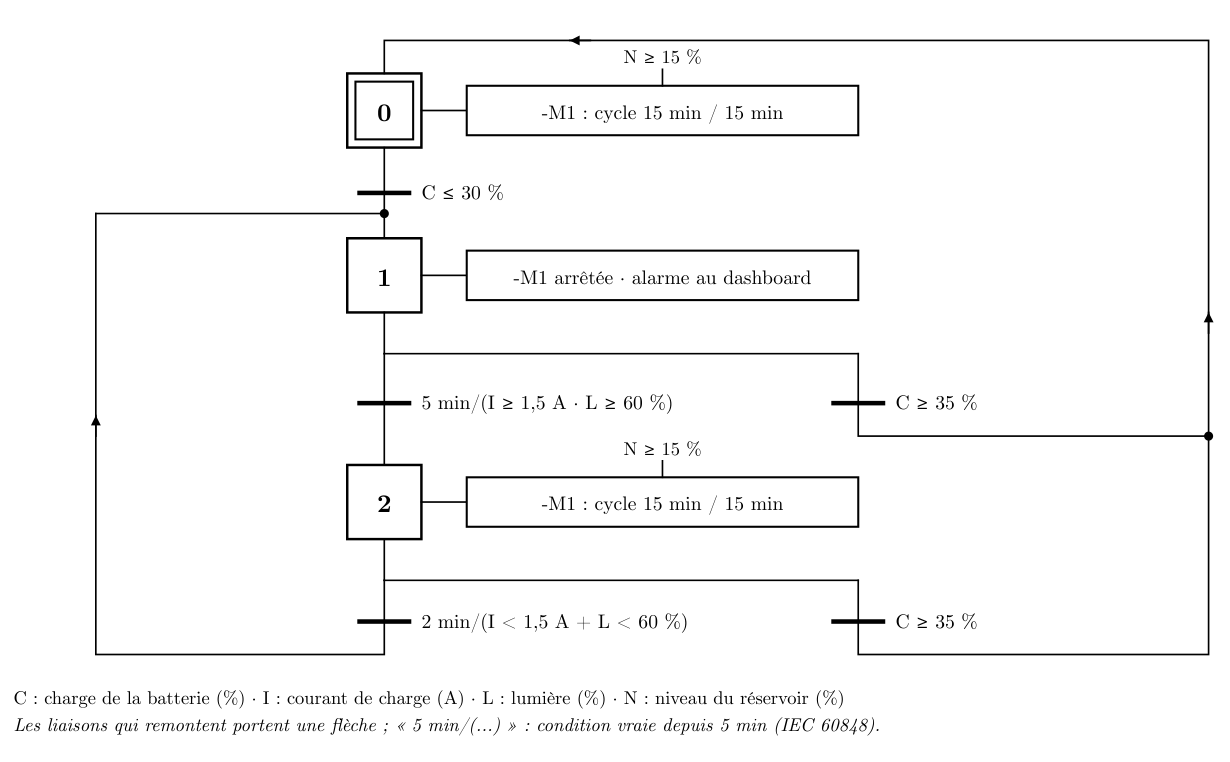
\includegraphics[width=0.9\textwidth]{img/inf/f_grafcet.png}
\schemacap{grafcet}{GRAFCET (IEC 60848) de la pompe principale -M1 : étape 0 normale, étape 1 coupée, étape 2 relancée par le soleil. Les seuils de 30 \% et 35 \% sont les valeurs conseillées, réglables dans le dashboard.}
\end{figure}

\subsubsection*{Le dosage selon le légume}

Pour le dosage, je veux éviter deux erreurs : verser trop de produit d'un coup, et corriger de nouveau avant que l'eau soit mélangée. Je choisis donc des doses courtes suivies d'une attente, comme on le ferait à la main. Les cibles changent avec le légume et son âge : plutôt que de les recopier dans le programme, je fais relire au Raspberry le tableau du dashboard, pour qu'il n'existe qu'une seule liste. Les essais me montrent aussi qu'il faut alterner engrais et pH$-$ quand les deux sont hors cible.

Les cibles de pH et d'EC dépendent du légume et de son stade de croissance, compté en jours depuis la plantation. Le tableau des légumes est écrit une seule fois, dans le dashboard ; le Raspberry le relit au démarrage, ce qui évite d'avoir deux listes différentes.

\begin{table}[H]
\centering
\small
\begin{tabularx}{\textwidth}{|l|l|c|c|}
\hline
\textbf{Légume} & \textbf{Stade (jours)} & \textbf{pH cible} & \textbf{EC cible (\unit{\micro S/cm})} \\
\hline
Salade (laitue) & Reprise (0--5) & 5,6 -- 6,0 & 1000 -- 1200 \\
 & Croissance des feuilles (5--22) & 5,6 -- 6,0 & 1200 -- 1600 \\
 & Pommaison (22--32) & 5,6 -- 6,0 & 1400 -- 1800 \\
 & Prête à récolter (32--42) & 5,6 -- 6,0 & 1400 -- 1800 \\
\hline
Tomate (cerise) & Reprise (0--7) & 5,8 -- 6,2 & 1500 -- 2000 \\
 & Croissance végétative (7--21) & 5,8 -- 6,2 & 1800 -- 2200 \\
 & Floraison (21--35) & 5,8 -- 6,3 & 2000 -- 2400 \\
 & Grossissement des fruits (35--60) & 5,8 -- 6,3 & 2200 -- 2800 \\
 & Récolte continue (60--88) & 5,8 -- 6,5 & 2400 -- 3000 \\
\hline
Poivron & Reprise (0--10) & 5,8 -- 6,2 & 1500 -- 1800 \\
 & Croissance végétative (10--30) & 5,8 -- 6,2 & 1800 -- 2200 \\
 & Floraison (30--45) & 5,8 -- 6,3 & 2000 -- 2300 \\
 & Grossissement des fruits (45--75) & 5,8 -- 6,3 & 2200 -- 2500 \\
 & Récolte (75--103) & 5,8 -- 6,3 & 2200 -- 2500 \\
\hline
\end{tabularx}
\caption{Cibles de pH et d'EC selon le légume et son stade.}
\end{table}

Les doses sont petites et espacées, pour laisser à l'eau le temps de se mélanger avant de mesurer à nouveau :

\begin{itemize}
\item on ne dose que si la pompe principale tourne depuis au moins 2 min (l'eau circule) et si le réservoir n'est pas presque vide ;
\item on attend \qty{10}{min} entre deux doses ;
\item EC trop basse : \qty{3}{s} d'engrais A, puis \qty{3}{s} d'engrais B ;
\item pH trop haut : \qty{2}{s} de pH$-$ ;
\item l'EC passe d'abord, car les engrais font bouger le pH ; si les deux sont hors cible, on alterne ;
\item au plus 12 doses par jour et par produit : au-delà, une sonde est sûrement défaillante.
\end{itemize}

L'organigramme suivant décrit le dosage, à chaque mesure.

\begin{figure}[H]
\centering
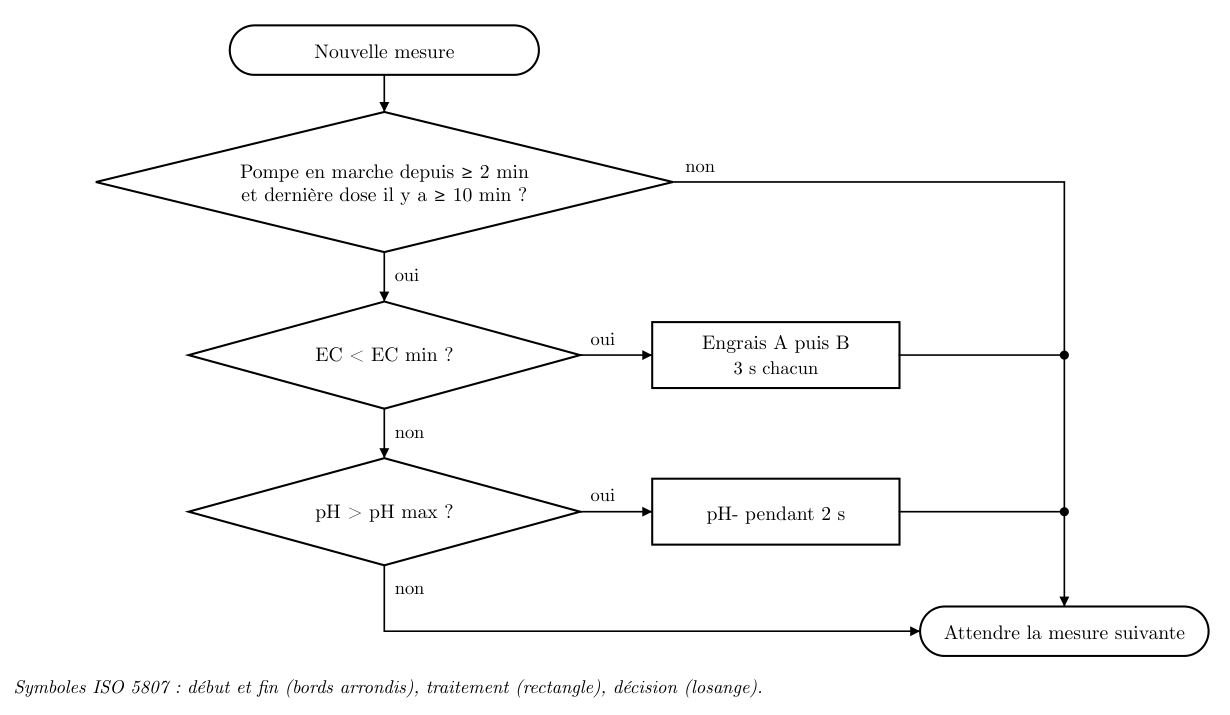
\includegraphics[width=0.85\textwidth]{img/inf/f_organigramme.png}
\schemacap{organi}{Organigramme (ISO 5807) du dosage, à chaque mesure. Pour rester lisible, il ne montre ni l'alternance entre engrais et pH$-$, ni la limite de 12 doses par jour.}
\end{figure}

\naturecalc{théorie (formule démontrée, valeurs de fiches techniques et hypothèses ; rien de mesuré)}
\begin{demonstration}[volume d'une dose]
\resultat{V_{\mathrm{engrais}} \approx \qty{5}{mL}\ \text{au plus}, \quad V_{\mathrm{pH-}} \approx \qty{3,3}{mL}\ \text{au plus}}
Les pompes péristaltiques\ix{8} débitent au plus $Q = \qty{100}{mL/min}$ (valeur de la fiche, à vide). Je calcule donc ici le volume maximal d'une dose. En divisant par $\qty{60}{s/min}$ :
\begin{align*}
Q &= \frac{\qty{100}{mL}}{\qty{60}{s}}\\
Q &\approx \qty{1,67}{mL/s}
\end{align*}
Le débit est constant : le volume versé pendant une durée $t$ (en secondes) est le produit du débit par la durée :
\[
V = Q \times t
\]
Pour chaque engrais, $t = \qty{3}{s}$ :
\begin{align*}
V &= \qty{1,67}{mL/s}\times\qty{3}{s}\\
V &\approx \qty{5}{mL}
\end{align*}
Pour le pH$-$, $t = \qty{2}{s}$ :
\begin{align*}
V &= \qty{1,67}{mL/s}\times\qty{2}{s}\\
V &\approx \qty{3,3}{mL}
\end{align*}
Le programme retire ces volumes du stock d'engrais saisi dans le dashboard, pour prévenir quand un flacon se vide. Ce sont des valeurs maximales : avec le débit en charge de \qty{80}{mL/min} supposé dans l'étude électrique (partie 5), une dose de \qty{3}{s} verse environ \qty{4}{mL} et une dose de \qty{2}{s} environ \qty{2,7}{mL}. La mesure M5 (partie 5) donnera le débit réel.
\end{demonstration}

\subsubsection*{Alertes et journal}

Un système autonome doit savoir prévenir quand il ne peut plus agir seul : réservoir vide, flacon d'engrais épuisé, pH trop bas alors qu'il n'y a pas de pH$+$. Je sépare les alarmes, qui demandent une action rapide, des simples avertissements, pour qu'on ne s'habitue pas à ignorer les messages rouges. À chaque mesure, le pilote dresse la liste des problèmes en cours. Les alarmes (en rouge) sont aussi notées dans le journal, avec les doses et les changements d'état :

\begin{table}[H]
\centering
\small
\begin{tabularx}{\textwidth}{|Y|l|Y|}
\hline
\textbf{Situation} & \textbf{Niveau} & \textbf{Message affiché} \\
\hline
Batterie sous le seuil de coupure & alarme & pompe arrêtée, reprise à \qty{35}{\percent} ou au soleil \\
\hline
Réservoir sous \qty{15}{\percent} & alarme & pompe et dosage arrêtés, ajouter de l'eau \\
\hline
12 doses dans la journée & alarme & dosage bloqué jusqu'au lendemain, vérifier la sonde \\
\hline
pH trop bas & à surveiller & pas de pH$+$ : corriger à la main \\
\hline
EC trop haute & à surveiller & ajouter de l'eau claire \\
\hline
Stock d'engrais sous \qty{0,2}{L} & à surveiller & flacon presque vide \\
\hline
Coupure sous \qty{30}{\percent} ou reprise sous \qty{35}{\percent} & conseil & valeurs conseillées pour protéger la batterie \\
\hline
Mode manuel & à surveiller & pilotage automatique en pause \\
\hline
\end{tabularx}
\caption{Alertes du pilote.}
\end{table}

